% Template for ICASSP-2019 paper; to be used with:
%          spconf.sty  - ICASSP/ICIP LaTeX style file, and
%          IEEEbib.bst - IEEE bibliography style file.
% --------------------------------------------------------------------------
\documentclass{article}
\usepackage{spconf,amsmath,graphicx,subfigure,float}
\usepackage{booktabs}
%...
% Example definitions.
% --------------------
\def\x{{\mathbf x}}
\def\L{{\cal L}}

 \graphicspath{{figs/}}
% Title.
% ------
\title{Speech denoising by parametric resynthesis}
%
% Single address.
% ---------------
\name{Soumi Maiti and Michael I Mandel}%\thanks{Thanks to XYZ agency for funding.}}
\address{The CUNY Graduate Center and Brooklyn College \\ New York, NY}
%
% For example:
% ------------
%\address{School\\
%	Department\\
%	Address}
%
% Two addresses (uncomment and modify for two-address case).
% ----------------------------------------------------------
%\twoauthors
%  {A. Author-one, B. Author-two\sthanks{Thanks to XYZ agency for funding.}}
%	{School A-B\\
%	Department A-B\\
%	Address A-B}
%  {C. Author-three, D. Author-four\sthanks{The fourth author performed the work
%	while at ...}}
%	{School C-D\\
%	Department C-D\\
%	Address C-D}
%
\begin{document}
%\ninept
%
\maketitle
%
\begin{abstract}

This work introduce a novel method for speech denoising that employs a parametric speech synthesis model. We propose to predict clean speech vocoder parameters from noisy speech using a neural network, and then use the vocoder to resynthesize predicted clean speech. In this way, the vocoder can produce high-quality speech and the model can predict features that are well-suited to speech enhancement tasks without having to explicitly represent complex phase. We compare, using objective metrics, against a matched text-to-speech system that is given the ground truth transcripts of the noisy speech. We show that our model is able to produce more natural speech because it has access to the prosody of the noisy speech. We then compare with two denoising systems, the oracle Wiener mask and a DNN-based mask predictor. Our model achieves better quality and comparable intelligibility in both subjective and objective measures because it is based on a high-quality synthesizer. We test speaker-dependence with two speakers and show that a single model can be used for multiple speakers.  
\end{abstract}
%
\begin{keywords}
Speech enhancement, synthesis, vocoder
\end{keywords}
%

\section{Introduction}
\label{sec:intro}
%We live in a noisy environment, 
The general approach of speech enhancement systems is to modify a noisy signal and make it more like the clean signal. The main problems for such systems is the over-suppression of the speech signal and under-suppression of the noise. Ideally, speech enhancement systems should remove noise completely without hampering the speech quality. An alternative approach to this are, speech synthesis systems which can produce high-quality speech from textual inputs. For example, statistical text to speech (TTS) systems map text to acoustic parameters of the speech signal and use a vocoder to then generate speech from these acoustic features. Statistical TTS systems train an acoustic model to learn the mapping from text to acoustic parameters of speech recordings. The most difficult part of this task, however, is predicting realistic prosody from pure text. In this work we propose combining these two approaches to capitalize on the strengths of each by predicting the acoustic parameters of clean speech from a noisy observation and then using a vocoder to synthesize the speech.  We show that this combined system can produce the vocoder synthesized high-quality and noise-free speech utilizing the prosody observed in the real noisy speech. 

We argue that the noisy speech signal has more information about the clean speech than pure text. Specifically, it is easier to model different speaker voice qualities and prosody from the noisy speech than from text. Hence, we can build a prediction model that takes noisy audio as input and accurately predicts acoustic parameters of clean speech. From the predicted acoustic features, we can generate clean speech using a speech synthesis vocoder. We train a neural network to learn the mapping from noisy speech features to clean speech acoustic parameters. Since we are creating a clean resynthesis of the noisy signal, the output speech quality will be higher than standard speech denoising systems and completely noise-free. We refer to the proposed model from this point as \emph{parametric resynthesis}.

In this paper, we show that the parametric resynthesis outperforms statistical TTS in terms of traditional speech synthesis objective metrics.  Next we subjectively evaluate the intelligibility and quality  of the resynthesized speech  and compare it with a mask predicted by a DNN-based system~\cite{WangTrainingTargetsSupervised2014} and the oracle Wiener mask~\cite{lim1979enhancement}. We show that the resynthesized speech is noise-free and has higher overall quality and intelligibility than both the oracle Wiener mask and the DNN-predicted mask. We also show that a single parametric resynthesis model can be used for multiple speakers.

%%%%%%%%%%%%%%%%%%%%%%%%%%%%%%%%%%%%%%%%%%%%%%%%%%%%%%%%%%%%%%%%%%%%%%%%%%%%%%%%%%%%%%%%%%%%%%%%%%%
\section{Related Work}
\label{sec:back}
Traditional speech synthesis systems are of two types, concatenative and parametric. In our previous works, \cite{mandel14c, maiti2017concatenative, maiti2018large, syed2018concatenative} we proposed concatenative synthesis systems for denoising speech. Though these models can generate high quality speech, they are speaker dependent and generally require a large dictionary of speech examples from that speaker. Alternatively, the current paper utilizes a parametric speech synthesis model, which more easily generalizes to combinations of conditions not seen explicitly in training examples.% using which it is trained. 

In terms of parametric resynthesis, Rethage et al.~\cite{rethage2018wavenet} built an end-to-end model to map noisy audio to explicit models of both clean speech and noise using a WaveNet-like~\cite{van2016wavenet} architecture.  Compared to this model, our denoising system is much simpler, as it does not require an explicit model of the observed noise in order to converge and needs much less data and time to train.  This simplicity comes from using the non-neural WORLD vocoder ~\cite{morise2016world}.

% In another work \cite{tamamori2017speaker}, authors describe use of WaveNet as a neural vocoder conditioned on traditional vocoder parameters. In \cite{adiga2018use}, authors improve on this work and suggest using different acoustic features for WaveNet vocoder for better result across speakers. In \cite{jin2018fftnet}, authors propose another neural vocoder FFTNet, which can generate better natural sounding speech. Both of these neural vocoders are speaker-dependent, hence using them for our speech denoising would constrain model to be speaker-dependent. So we limit our experiments with traditional non-neural WORLD  vocoder. 


%%%%%%%%%%%%%%%%%%%%%%%%%%%%%%%%%%%%%%%%%%%%%%%%%%%%%%%%%%%%%%%%%%%%%%%%%%%%%%%%%%%%%%%%%%%%%%%%%%%

\begin{figure}[htb]
\begin{minipage}[b]{1.0\linewidth}
  \centering
  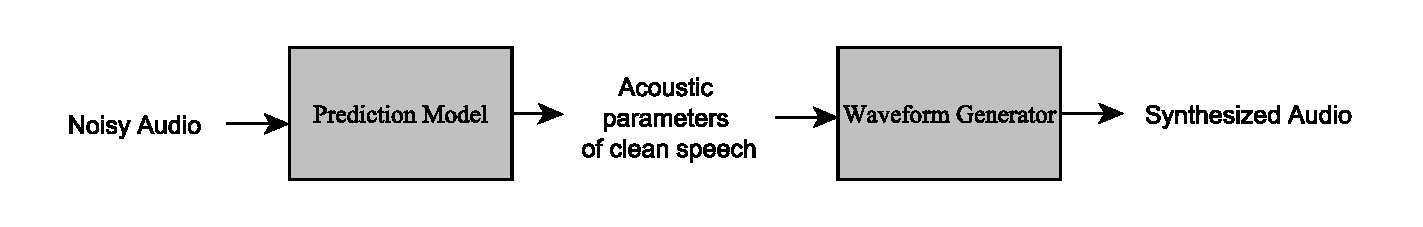
\includegraphics[trim={0.15cm 0 0.35cm 0},clip, width=1.0\textwidth,height=1.4cm]{model.eps}
%  \vspace{2.0cm}
%  \centerline{(a) Result 1}\medskip
\end{minipage}
\caption{Vocoder denoising model}
\label{fig:model}
\end{figure}

%%%%%%%%%%%%%%%%%%%%%%%%%%%%%%%%%%%%%%%%%%%%%%%%%%%%%%%%%%%%%%%%%%%%
\section{Model overview }
\label{sec:mod_ovr}
Parametric resynthesis consists of two stages: prediction and synthesis as shown in Fig \ref{fig:model}. We first train a prediction model with noisy audio features as input and clean acoustic features as output labels. The second stage is to resynthesize audio using the vocoder from the predicted acoustic features.

%%%%%%%%%%%%%%%%%%%%%%%%%%%%%%%%%%%%%%%%%%%%%%%%%%%%%%%%%%%%%%%%%%%%%%%%%%%%%%%%%%%%%%%%%%%%%%%%%%%
\subsection{Synthesis from acoustic features}
\label{sub:synth}
For the synthesis from acoustic features, the WORLD vocoder is used. This vocoder allows both the encoding of speech audio into acoustic parameters and the decoding of acoustic parameters back into audio with very little loss of speech quality.  The advantage is that these parameters are much easier to predict using neural network prediction models.  We use the encoding of clean speech to generate our training targets and the decoding of predictions to generate output audio.  The WORLD vocoder is incorporated into the Merlin neural network-based speech synthesis system \cite{wu2016merlin}, and we utilize Merlin's training targets and losses for our model.

% Vocoder is traditionally used in communication systems to generate a compact representation of audio, so that audio can be transmitted with less information. It consists of two parts, encoder, that converts speech to compact representation and decoder, that receives the representation and generates speech waveform. Here, the compact representation are set of acoustic features. In vocoder speech denoising model, we predict acoustic features of clean speech and then use decoder side of vocoder to generate resynthesis. 

%%%%%%%%%%%%%%%%%%%%%%%%%%%%%%%%%%%%%%%%%%%%%%%%%%%%%%%%%%%%%%%%%%%%%%%%%%%%%%%%%%%%%%%%%%%%%%%%%%%
%\subsection{Relation to speech synthesis}
%\label{sub:speech_synth}

% Statistical TTS systems has two ends, front-end, that produces linguistic specification from text and back-end, that predicts acoustic features from linguistic specifications. Our prediction model is similar to the back-end of statistical TTS system in output, except that it uses different input features.  There is more information in noisy audio about the acoustic features of the clean audio signal than simple text.

%%%%%%%%%%%%%%%%%%%%%%%%%%%%%%%%%%%%%%%%%%%%%%%%%%%%%%%%%%%%%%%%%%%%%%%%%%%%%%%%%%%%%%%%%%%%%%%%%%%
\subsection{Prediction model}
\label{sub:model}
The prediction model is a neural network that takes as input log mel spctra of the noisy audio and predicts clean speech acoustic features at a fixed frame rate. Clean speech acoustic parameters are extracted from the encoder of the WORLD vocoder. The encoder outputs three acoustic parameters: i) spectral envelope, ii) log fundamental frequency (F0) and iii) aperiodic energy of the spectral envelope. Fundamental frequency is used to predict voicing, a parameter required for the vocoder. All the three features are concatenated with their first and second derivatives and used as the targets of the prediction model. There are 60 features from spectral envelope, 5 from band aperiodicity, 1 from F0 and a Boolean flag for the voiced or unvoiced decision. The prediction model is then trained to minimize the mean squared error loss from prediction and ground truth. This architecture is similar to the acoustic modelling of statistical TTS. We first use a feed-forward DNN as the core of the prediction model, then we use LSTMs~\cite{hochreiter1997long} for better sequence-to-sequence mapping. Input features are concatenated with neighbouring frames ($\pm 4$) for the feed-forward DNN.
%%%%%%%%%%%%%%%%%%%%%%%%%%%%%%%%%%%%%%%%%%%%%%%%%%%%%%%%%%%%%%%%%%%%%%%%%%%%%%%%%%%%%%%%%%%%%%%%%%%
\begin{table*}[bt]
    \centering
    \begin{tabular}{ccc c ccc} \toprule
     & \multicolumn{2} {c} {\bfseries Spectral Distortion } & \phantom{abc} & \multicolumn{3} {c} {\bfseries $F0$ measures} \\ 
     \cmidrule{2-3}  \cmidrule{5-7}
     System                     & MCD (dB) & BAPD (dB) && RMSE (Hz) & CORR & VUV \\ 
    \midrule
      PR-clean      & 2.68  & 0.16      && 4.95 & 0.96 & 2.78\% \\
      \midrule
    TTS (DNN)                   & 5.28  & 0.25       && 13.06   & 0.71 & 6.66\% \\
    TTS (LSTM)                  & 5.05  & 0.24       && 12.60    & 0.73 & 5.60\% \\
    PR (DNN)  & 5.07 & 0.19     && 8.83 & 0.93 & 6.48\% \\
    PR (LSTM) & \textbf{4.81} & \textbf{0.19}     && \textbf{5.62} & \textbf{0.95} & \textbf{5.27\%} \\
    \bottomrule
    \end{tabular}
    \caption{TTS objective measures. For MCD, BAPD, RMSE, and VUV lower is better, for CORR higher is better.}
    \label{tab:obj_eval_tts}
\end{table*}
%mean cepstral distortion (MCD), band aperiodicity (BAPD), root mean square error (RMSE), voiced-unvoiced error rate (VUV), and correlation (CORR). For MCD, BAPD, RMSE, and VUV lower is better, for CORR higher is better.
\section{Experiments}
\label{sec:expr}
\subsection{Dataset}
\label{ssec:data}
The noisy dataset is generated by adding environmental noise to the CMU arctic speech dataset \cite{kominek2004cmu}. The arctic dataset contains four versions of the same sentences spoken by four different speakers, with each version having 1132 sentences. The speech is recorded in studio environment. The sentences are taken from different parts of project Gutenberg and are phonetically balanced. To make the data noisy, we add environmental noise from the CHiME-3 challenge \cite{BarkerthirdCHiMEspeech2015}. The noise was recorded in four different environments: street, pedestrian walkway, cafe, and bus interior. Six channels are available for each noisy file, we treat all channels as separate noise source. We mix clean speech with one of the random noise files starting from a random offset with a constant gain of 0.95. The signal-to-noise ratio (SNR) of the noisy files ranges from -6~dB to 21~dB, with average being 6~dB. The sentences are 2 to 13 words long, with a mean length of 9 words. We mainly use a female speech corpus (``slt'') for our experiments. A male (``bdl'') voice is used to test the speaker-dependence of the system. The dataset is partitioned into 1000-66-66 as train-dev-test. 
%
%We use the speech synthesis toolkit Merlin \cite{wu2016merlin} for the implementation of our model and the TTS baseline. The WORLD vocoder \cite{morise2016world} is used for waveform generation, which is distributed with the Merlin toolkit. 
The input and output features are extracted with a window size of 64~ms at a 5~ms hop size. 
%Log mel spectra are extracted from noisy audio and used as input features for the prediction model. Output feature labels (spectral envelope, band aperiodicity and F0) are generated by WORLD.  

\subsection{Evaluation}
\label{ssec:eval}
We evaluate two aspects of the parametric resynthesis system.
Firstly, we compare speech synthesis objective metrics like spectral distortion and F0 prediction errors with a TTS system. This objectifies the performance of our model as compared to TTS. Secondly, we compare the intelligibility and quality of the speech generated by paramteric resynthesis (PR) against two speech enhancement systems, ideal-ratio mask and oracle Wiener mask (OWM) \cite{lim1979enhancement,scalart1996speech}. The ideal ratio mask is predicted from DNN (DNN-IRM) \cite{WangTrainingTargetsSupervised2014} and trained with the same data as PR. OWM uses knowledge of true speech to estimate the Wiener mask. Hence, OWM places an upper bound on the performance achievable by the mask based enhancement systems. 

A limitation of the proposed method is that vocoded speech can sound mechanical or muffled at times. So we encode and decode clean speech with the vocoder and estimate loss in intelligibility and quality attributable to the vocoder alone, which we show is minimal. We call this system vocoder-encoded-decoded (VED). Moreover, we also measure the performance of a DNN that predicts vocoder parameters from clean speech as a more realistic upper bound on our speech denoising system. This is the PR model with clean speech as input, referred to as PR-clean.

%\subsection{Systems}
%\label{ssec:sys}
%We compare the parametric resynthesis system with five other systems in different %combinations,
%\begin{itemize}
%\itemsep0em 
%\item VED : Use vocoder to encode and decode clean speech. This system quantifies the loss in quality and intelligibility attributable to the vocoder alone, which we to be minimal.
%\item PR-clean: This is the parametric resynthesis model using clean speech as input. This system provides a tighter upper bound on the performance achievable by the real parametric resynthesis system.
%\item PR: Our parametric resynthesis system, where we predict acoustic features of clean speech from noisy speech and generate audio using the vocoder.
%\item TTS: Traditional statistical text-to-speech speech given the true transcript of the noisy speech.  It is trained on the same data and uses a similar acoustic model DNN configuration to the parametric resynthesis system. 
%\item Oracle Wiener mask (OWM) \cite{lim1979enhancement,scalart1996speech}: Places an upper bound on the performance achievable with mask-based enhancement by using knowledge of the true speech.
%\item DNN-predicted Ideal Mask Ratio (DNN-IRM) %\cite{WangTrainingTargetsSupervised2014}: Mask-based speech enhancement system, trained on the same training data as vocoder denoising system.
%\end{itemize}
%We also compare the results with reference clean and noisy signals.


\begin{table*}[bt]
    \centering
    \begin{tabular}{cccccccccc} \toprule
& \multicolumn{2}{c}{\bfseries Speakers} & \phantom{a} & \multicolumn{2}{c}{\bfseries Spectral Distortion} & \phantom{a}& \multicolumn{3}{c}{\bfseries F0 measures}\\
\cmidrule{2-3}  \cmidrule{5-6}  \cmidrule{8-10}
    Model & Train & Test && MCD & BAPD && RMSE & CORR & UUV \\
     \midrule
    PR & slt      & slt    && 4.81 & 0.19 && 5.62  & 0.95 & 5.27\% \\
    PR & slt+bdl & slt    && 4.91 & 0.20 && 8.36  & 0.92 & 6.50\%\\
    PR & bdl      & bdl     && 5.40 & 0.21 && 9.67 & 0.82 & 12.34\%\\
    PR & slt+bdl & bdl    && 5.19 & 0.21 && 10.41  & 0.82 & 12.17\%\\
    %PR-(slt+bdl) & slt+bdl  & 64 & 4.96 & 0.20 && 9.22  & 0.96 & 8.89\%\\ 
    \bottomrule
    \end{tabular}
    \caption{TTS objective measures for multi-speaker parametric resynthesis models compared to single speaker model on two 32-utterance single-speaker test sets. }
    \label{tab:speaker}
\end{table*}


%%%%%%%%%%%%%%%%%%%%%%%%%%%%%%%%%%%%%%%%%%%%%%%%%%%%%%%%%%%%%%%%%%%%%%%%%%%%%%%%%%%%%%%%%%%%%%
\subsection{TTS objective measures}
First, we evaluate TTS objective measures of PR, PR-clean with TTS system. We train a feedforward DNN  with 4 layers of 512 width system with tanh activation function and a LSTM  system with 2 layers of width 512. We use adam optimization and early stopping regularization. For TTS system inputs, we use ground truth transcription of noisy speech. As both TTS and PR are predicting acoustic features, we measure erros in the prediction. We measure mel cepstral distortion (MCD) and band aperiodicity distortion (BAPD), F0 root mean square error (RMSE), Pearson correlation (CORR) of F0 and classification error in voiced-unvoiced decisions (VUV) with ground truth acoustic features. The results are reported in Table~\ref{tab:obj_eval_tts}.

Results from PR-clean shows that speech with very low spectral distortion and F0 error can be achieved from clean speech. More importantly we see from Table \ref{tab:obj_eval_tts} that PR performs considerably better than TTS systems. It is also interesting to note that the F0 measures, RMSE and Pearson correlation are significantly better in the parametric resynthesis system than TTS. This proves our claim that it is easier to predict acoustic features from noisy speech than from text. We observe that the LSTM performs best and is used for the following experiments. 



%%%%%%%%%%%%%%%%%%%%%%%%%%%%%%%%%%%%%%%%%%%%%%%%%%%%%%%%%%%%%%%%%%%%
\subsubsection{Evaluating multiple speaker model}
Next we train a PR model with speech from two speakers and test its effectiveness on both speaker datasets. We first train two single-speaker PR models using the slt (female) and bdl (male) data in the CMU arctic dataset. Then we train a new PR model with speech from both speakers. We measure the objective metrics on both datasets to understand how well a single model can be generalized for both speakers. 

These objective metrics are reported in Table~\ref{tab:speaker}, from which we observe that the single-speaker model slightly out-performs the multi-speaker model. On bdl dataset, however, the multi-speaker model performs better than the single-speaker model in predicting voicing decision and MCD; and scores the same in BAPD and F0 correlation, but does worse on F0 RMSE. %Hence, the parametric resynthesis system is able to predict acoustic features of both speakers simultaneously.
These results show that the same model can be used for multiple speakers.  In a future work we will investigate the degree to which a single model can generalize to completely unseen speakers.


%%%%%%%%%%%%%%%%%%%%%%%%%%%%%%%%%%%%%%%%%%%%%%%%%%%%%%%%%%%%%%%%%%%%
\subsection{Speech enhancement objective measures}

%In this section we compare the parametric resynthesis system with two comparison speech enhancement systems. The first comparison system is the oracle Wiener mask, which places an upper bound on the performance of any mask-based speech enhancement system by using knowledge of the true clean speech. The second comparison system is the ideal ration mask predicted by a DNN, trained on same data as our model. 
We measure objective intelligibility with short-time-objective-intelligibility (STOI) \cite{taal2010short} and objective quality with perceptual evaluation of speech quality (PESQ) \cite{rix2001perceptual}. We also measure STOI and PESQ of clean, noisy, VED, TTS, PR-clean for reference. The results are reported in Table~\ref{tab:obj_denoise}. 


VED files are very high in objective quality and intelligibility. This shows that the vocoder loss is negligible compared to the clean signal and much higher than the speech enhancement systems. The PR-clean system scores slightly lower in intelligibility and quality than VED. The TTS system scores very low, but this can be explained by the fact that the objective measures compare the output to original clean signal. 

For speech denoising systems, parametric resynthesis outperforms both the OWM and the predicted IRM in objective quality score.  While the oracle Wiener mask is an upper bound on mask-based speech enhancement, it does degrade the quality of the speech by attenuating and damaging speech regions where there is speech present, but the noise is louder. Parametric resynthesis also achieves higher intelligibility than the predicted IRM system but slightly lower intelligibility than the oracle Wiener mask. 

%%%%%%%%%%%%%%%%%%%%%%%%%%%%%%%%%%%%%%%%%%%%%%%%%%%%%%%%%%%%%%%%%%%%
\begin{table}[bt]
    \centering
\begin{tabular}{ccc}
\toprule
Model & PESQ & STOI \\
\midrule
Clean               & 4.50 & 1.00 \\
VED  & 3.39 & 0.93 \\
PR-clean  & 2.98 & 0.92\\
OWM      & 2.27 & 0.92 \\
Noisy               & 1.88 & 0.88\\
TTS                 & 1.33 & 0.08\\
\midrule
%Wiener mask  (priori SNR)     & 2.26 & 0.88 \\
PR &  2.43 & 0.87 \\
DNN-IRM          & 2.26 & 0.80\\
\bottomrule
\end{tabular}
\caption{Speech enhancement objective metrics: Intelligibility and Quality, higher is better.}
\label{tab:obj_denoise}
\end{table}
%,


%%%%%%%%%%%%%%%%%%%%%%%%%%%%%%%%%%%%%%%%%%%%%%%%%%%%%%%%%%%%%%%%%%%%
\begin{figure}[tb]
\begin{minipage}[b]{0.95\linewidth}
  \centering
  \centerline{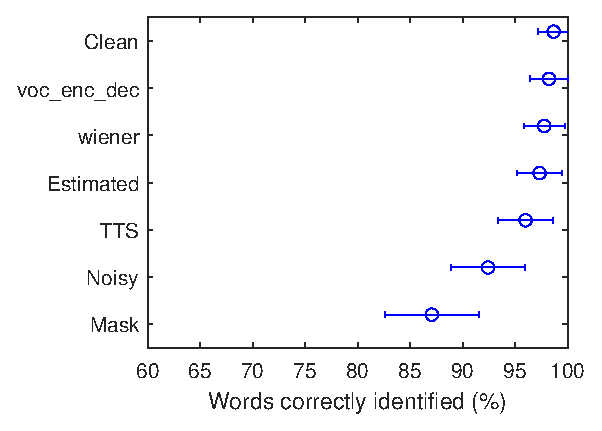
\includegraphics[width=.75\linewidth, trim={0 0.6cm
0 0},clip]{00-intel.eps}}
%  \vspace{1.5cm}
  %\centerline{Subjective intelligibility}\medskip
  \caption{Subjective intelligibility: percentage of correctly identified words}
 \label{fig:intel}
\vspace{0.4cm}
\end{minipage}
%\end{figure}
%\begin{figure}
\begin{minipage}[b]{0.95\linewidth}
  \centering
  \centerline{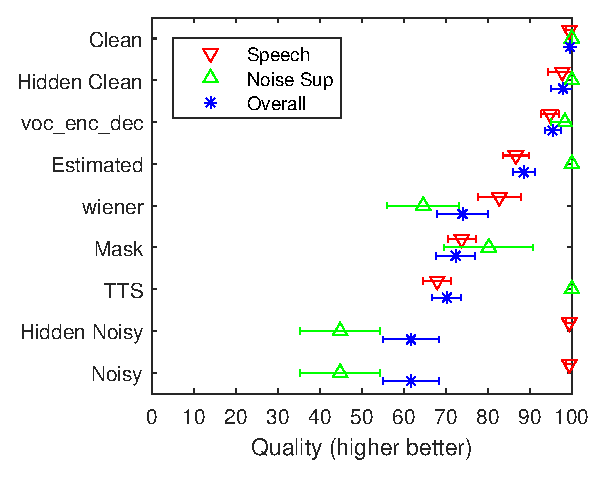
\includegraphics[width=.8\linewidth,  trim={0 0.61cm
0.4 0},clip]{01-qual.eps}}
%  \vspace{1.5cm}
  %\centerline{(c) Subjective quality results over 2 subjects}\medskip
  \caption{Subjective quality, higher is better.}
  \label{fig:qual}
\end{minipage}
\end{figure}

\subsection{Subjective Intelligibility and Quality}

Finally we evaluate the subjective intelligibility and quality of PR and compare it with OWM, DNN-IRM, PR-clean, and the ground truth clean and noisy speech. From 66 test sentences we chose 12, with 4 sentences from each of three groups: SNR $< 0$ dB, $0$~dB $\leq$ SNR $< 5$~dB, and $5$~dB $\leq$ SNR. In preliminary listening tests, we observe that PR-clean files sounds as good as VED, so we included only PR-clean.  This resulted in a total of 84 files (12 sentences times 7 versions).

For the subjective intelligibility test, subjects were presented with all 84 sentences in a random order and were asked to transcribe the words that they heard in each one.  Three subjects listened to the files. A list of all of the words was given to the subjects in alphabetical order, but they were asked to write what they hear. We measure the percentage of words correctly identified averaged of over all files and show in Fig \ref{fig:intel}. Intelligibility is very high ($>90\%$) in all systems, including noisy. PR-clean achieves intelligibility as good as clean speech. OWM, PR and noisy speech intelligibility were same and very close to clean speech. This shows that PR achieves intelligibility as high as the oracle Wiener mask.

The speech quality test follows the Multiple Stimuli with Hidden Reference and Anchor (MUSHRA) paradigm \cite{MUSHRA}. Subjects were presented with all seven of the versions of a given sentence together in a random order without identifiers, along with reference clean and noisy versions. The subjects rated the speech quality, noise reduction quality, and overall quality of each version in a range of 1 to 100, with higher scores denoting better quality. Three subjects participated and results are shown in Fig \ref{fig:qual}.
From the results, we see that PR system achieves perfect noise suppression quality, proving the system is noise-free. PR also achieves better overall quality than IRM and OWM. Among the speech enhancement systems oracle Wiener mask achieves best speech quality, followed by PR. Thus, PR system achieves better quality in all three measures than DNN-IRM, and better noise suppression and overall quality than oracle Wiener mask. We also observe a small loss in noise suppression and overall quality for PR-clean. 

\section{Conclusion}
\label{sec:concl}
In this paper we introduce a novel speech denoising system inspired by the speech synthesis techniques from statistical TTS. The proposed  parametric resynthesis (PR) system predicts acoustic parameters of clean speech from noisy speech directly, and then uses a \emph{vocoder} to synthesize ``cleaner'' speech. We show that this model outperforms statistical TTS by utilizing prosody from the noisy speech. It outperforms the oracle Wiener mask in quality by reproducing the entire speech signal, while providing comparable intelligibility. As future work, we want to explore the extent of speaker-independence that is achievable with this system and explore other kinds of inputs like filtered and degraded speech~\cite{mandel15d}, and even neural activations in the auditory cortex~\cite{AkbariReconstructingintelligiblespeech2018}. 
%\vfill \pagebreak

%\section{REFERENCES}
%\label{sec:refs}

% References should be produced using the bibtex program from suitable
% BiBTeX files (here: strings, refs, manuals). The IEEEbib.bst bibliography
% style file from IEEE produces unsorted bibliography list.
% -------------------------------------------------------------------------
\bibliographystyle{IEEEbib}
\bibliography{refs}

\end{document}
